\documentclass[a4paper]{article}

%% Language and font encodings
\usepackage[english]{babel}
\usepackage[T1]{fontenc}

%% Sets page size and margins
\usepackage[a4paper,top=3cm,bottom=2cm,left=3cm,right=3cm,marginparwidth=1.75cm]{geometry}

%% Useful packages
\usepackage{amsmath}
\usepackage{graphicx}
\usepackage[colorlinks=true, allcolors=blue]{hyperref}

\title{Neural Networks Task 5}
\author{Jens, Mellberg, 11806523\\
		Group partner: Lassi, Lehtonen 11805955}



\begin{document}
\maketitle



\section{Training an LSTM with one hidden layer}

We begin the training with a learning rate of 0.0001 and batch size 40.
We find that adjusting the batch size does not improve the performance of our network, so we let the batch size remain 40.
However, increasing the learning rate by small increments seems to improve the performance and decrease the convergence time.
As seen in the plots, the convergence time decreases and we find our optimal performance when the learning rate is 0.00035.
Increasing the learning rate more, the performance of our network will decrease.
We conclude that the optimal learning rate for our network is 0.00035 with the batch size of 40.


\section{Training the same LSTM, but now with ADAM}

Our training begins with a learning rate of 0.0001 and default values for other parameters.
As seen in the plots, it requires 45 epochs for convergence. We proceed by increasing the learning rate gradually.
The evolution of the training/validation error is depicted in the provided plots. We reach a good performance at learning rate 0.0025.
We perform our ten learning runs with these parameters, the results are shown in the table below.\\\\
Increasing the learning rate obviously improves performances because the network will take bigger steps when decreasing the error. 

\begin{center}
	    \begin{tabular}{ |c|c|} 
 	        \hline
	        \textbf{Run } & \textbf{Epochs}  \\
	        \hline
	        1 & 2\\
 	        2 & 2\\
 	        3 & 2\\
 	        4 & 2\\
 	       5& 1\\
		6 & 2\\
		7 & 2\\
		8 & 2\\
		9 & 2\\
		10 & 2\\
		\hline
		\textbf{Mean} & 1.9\\
		\hline
		\textbf{STD} & 0.316228\\
 	        \hline
        \end{tabular}
    \end{center}




\begin{figure}[h]
\caption{Gradiant descent with learning rate 0.0001}
\centering
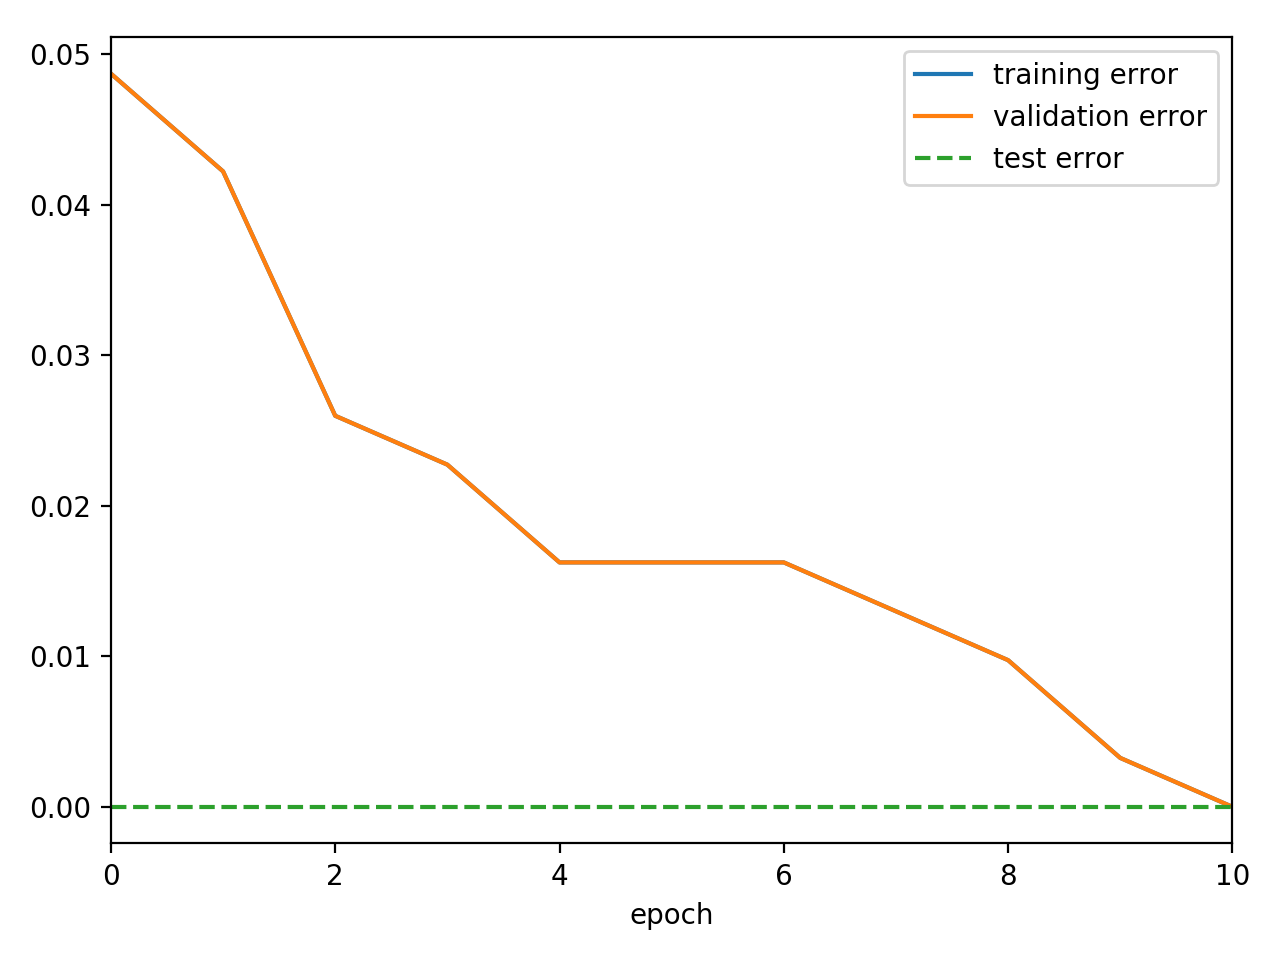
\includegraphics[width=15cm, height=12cm]{GD_LR0001}
\end{figure}

\begin{figure}[h]
\caption{Gradiant descent with learning rate 0.0002}
\centering
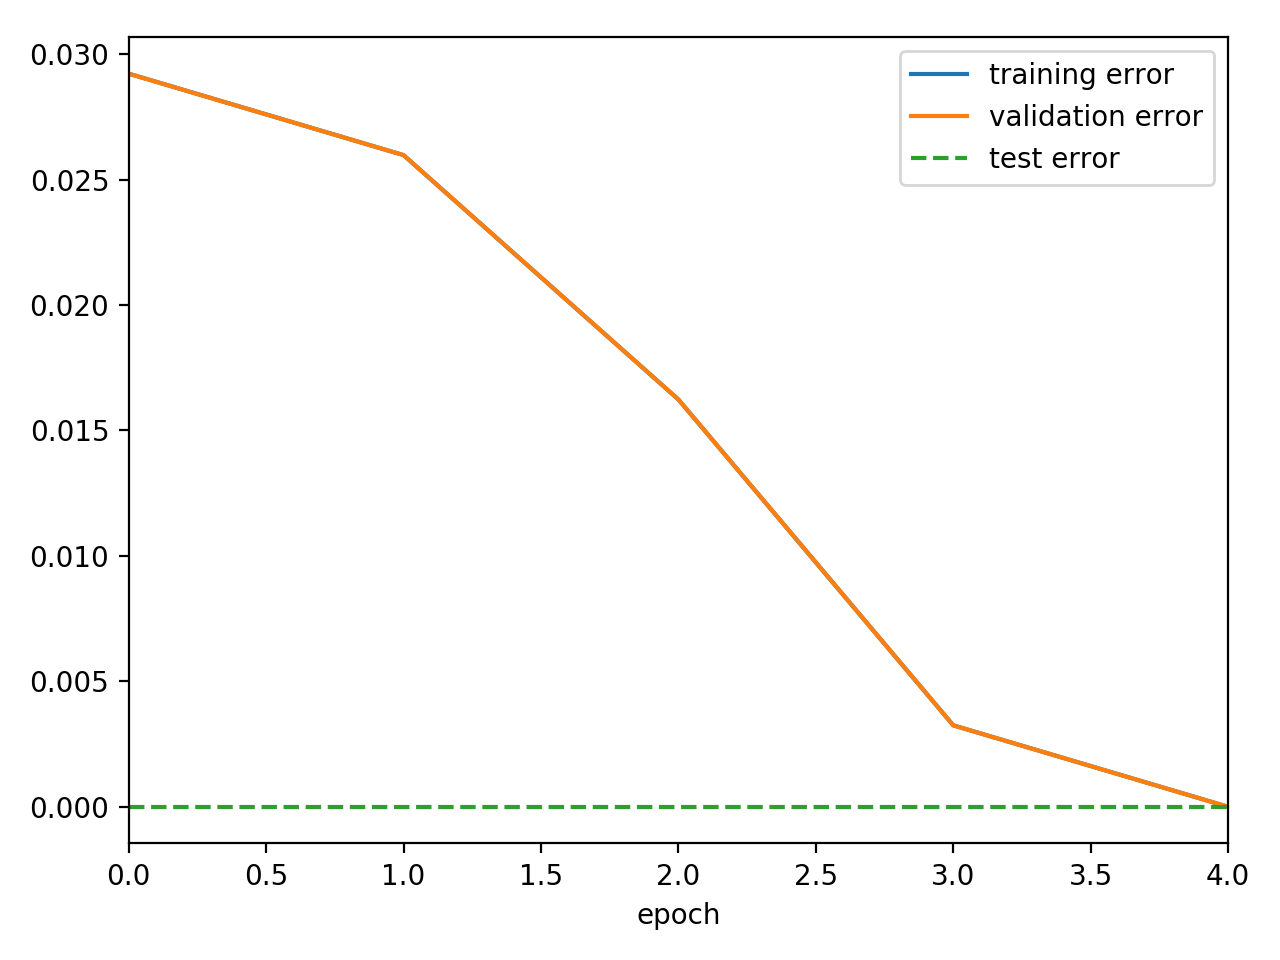
\includegraphics[width=15cm, height=12cm]{GD_LR0002}
\end{figure}

\begin{figure}[h]
\caption{Gradiant descent with learning rate 0.0003}
\centering
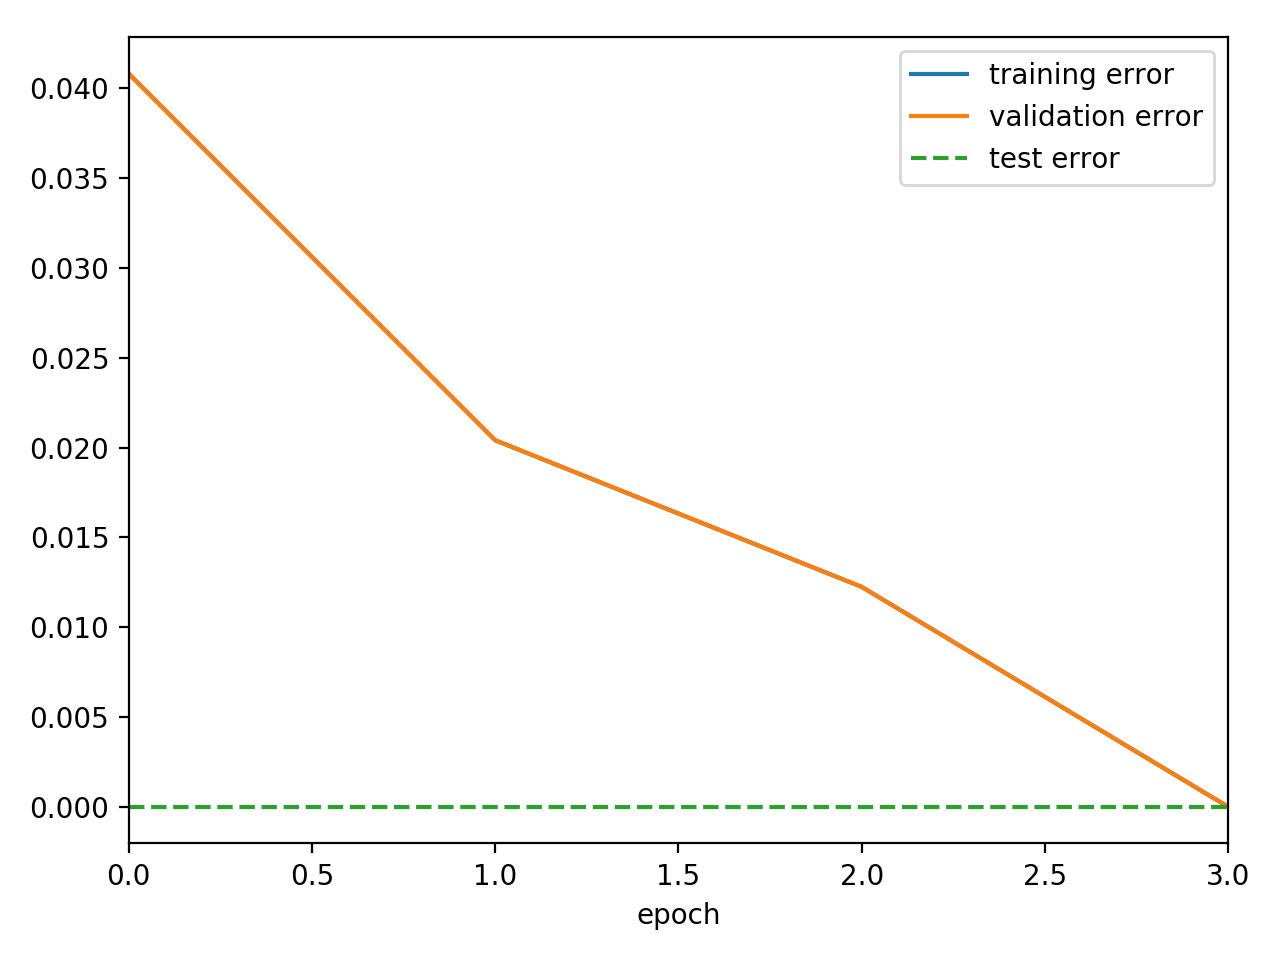
\includegraphics[width=15cm, height=12cm]{GD_LR0003}
\end{figure}

\begin{figure}[h]
\caption{Gradiant descent with learning rate 0.00035}
\centering
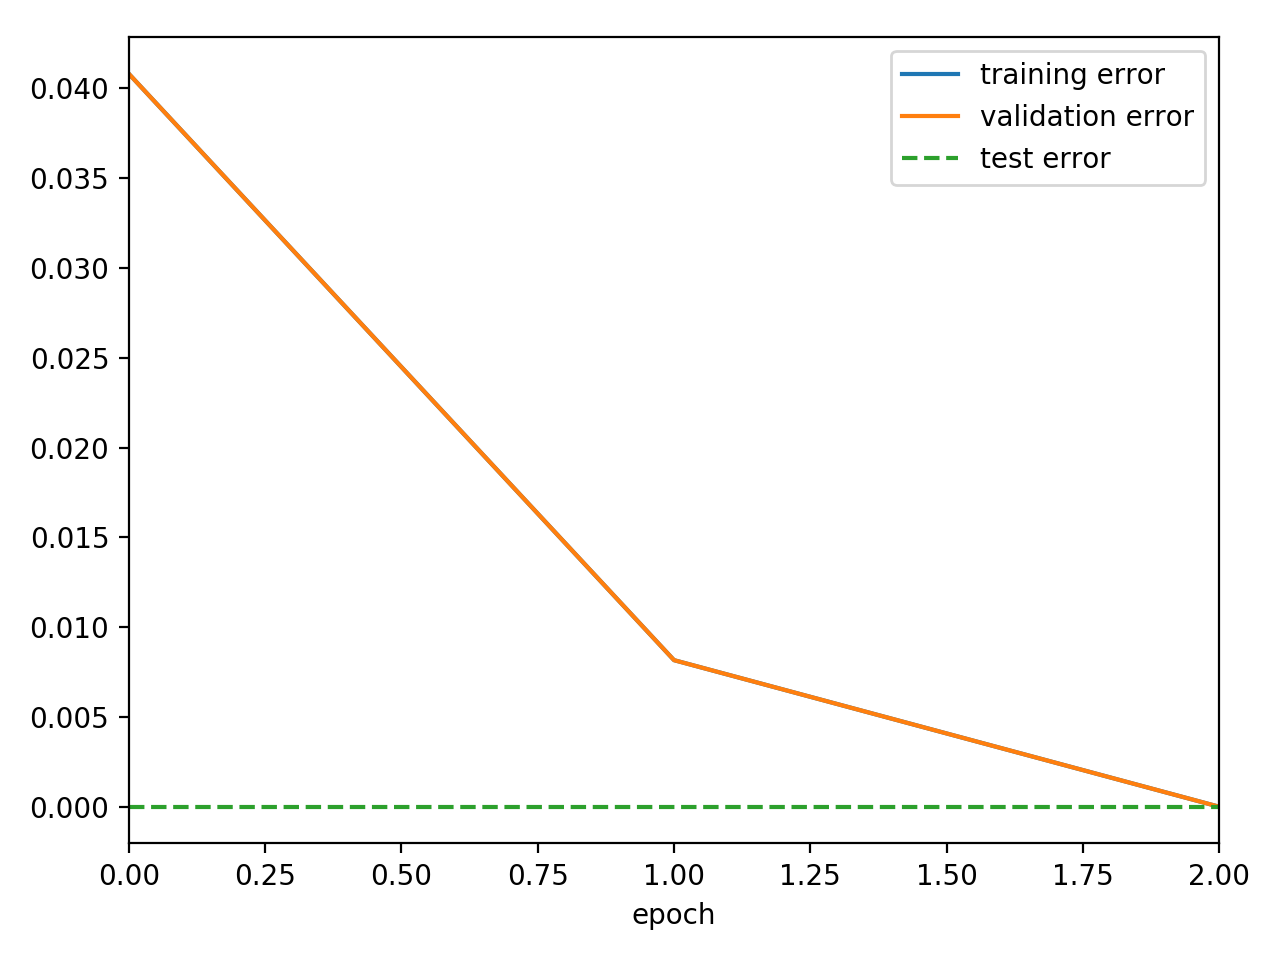
\includegraphics[width=15cm, height=12cm]{GD_LR00035}
\end{figure}

\begin{figure}[h]
\caption{ADAM with learning rate 0.0001}
\centering
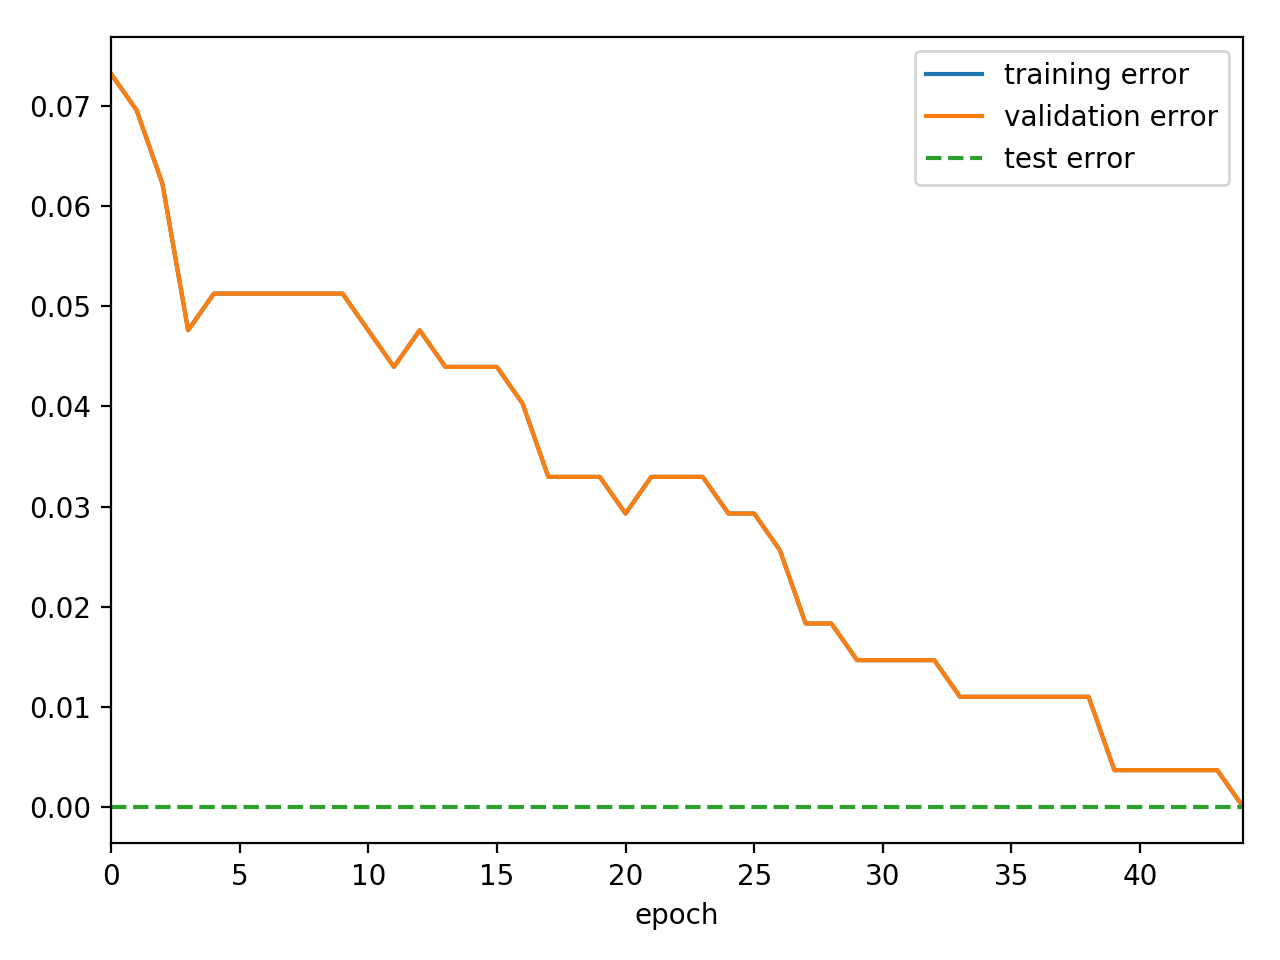
\includegraphics[width=15cm, height=12cm]{AD_LR0001}
\end{figure}

\begin{figure}[h]
\caption{ADAM with learning rate 0.0002}
\centering
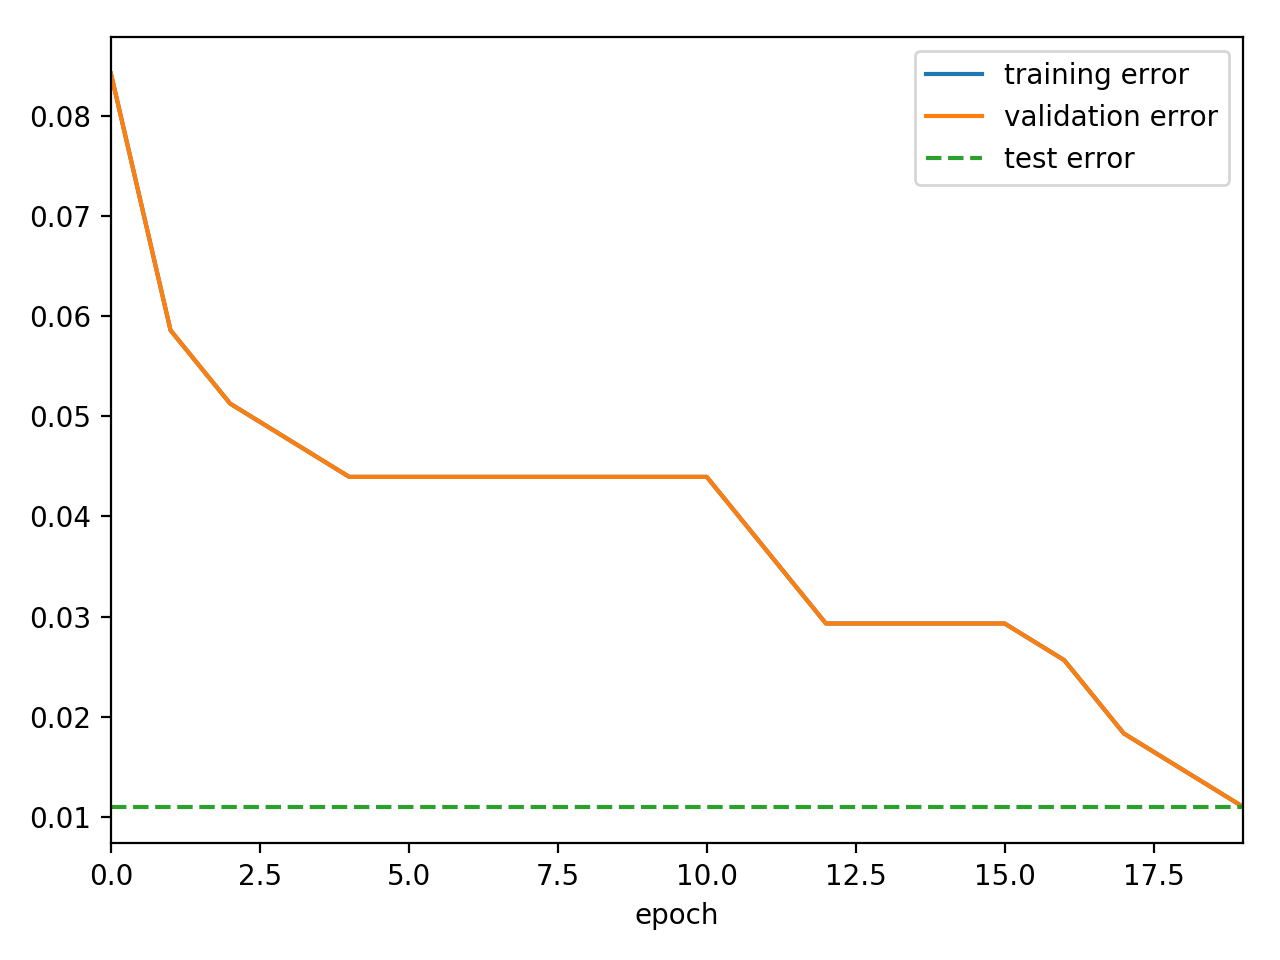
\includegraphics[width=15cm, height=12cm]{AD_LR0002}
\end{figure}

\begin{figure}[h]
\caption{ADAM with learning rate 0.0004}
\centering
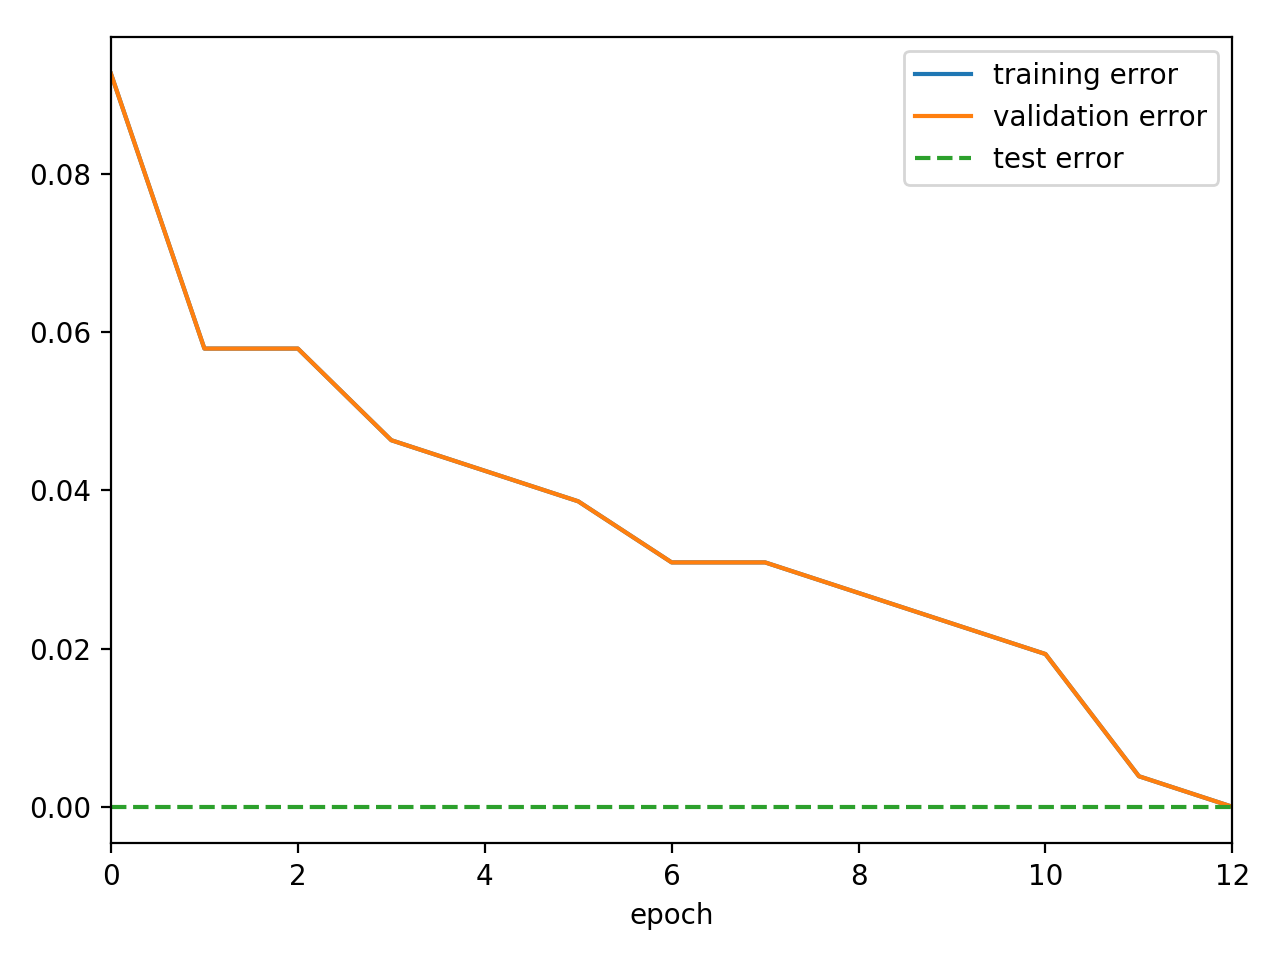
\includegraphics[width=15cm, height=12cm]{AD_LR0004}
\end{figure}

\begin{figure}[h]
\caption{ADAM with learning rate 0.0006}
\centering
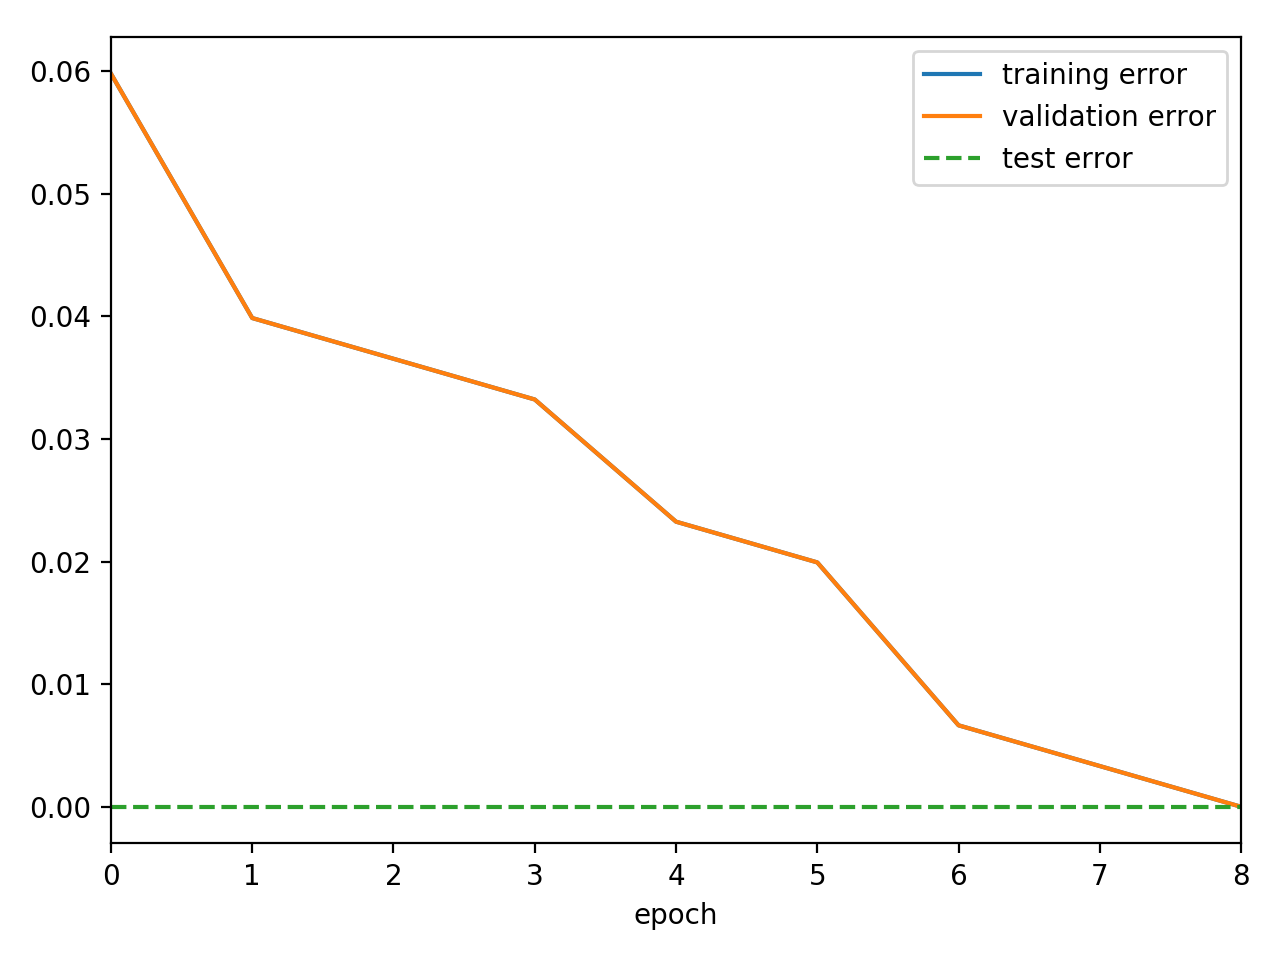
\includegraphics[width=15cm, height=12cm]{AD_LR0006}
\end{figure}

\begin{figure}[h]
\caption{ADAM with learning rate 0.0009}
\centering
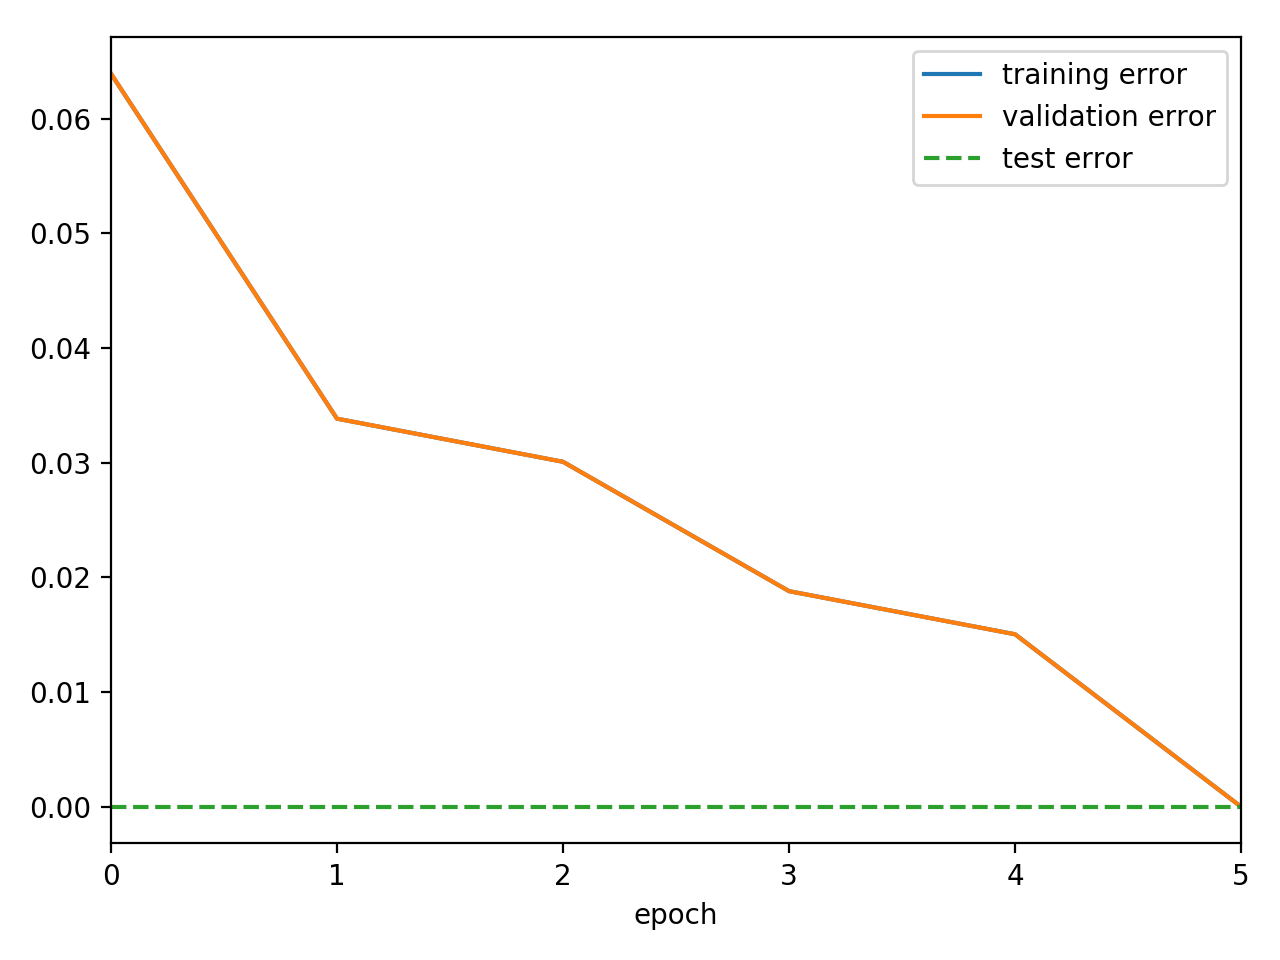
\includegraphics[width=15cm, height=12cm]{AD_LR0009}
\end{figure}

\begin{figure}[h]
\caption{ADAM with learning rate 0.0015}
\centering
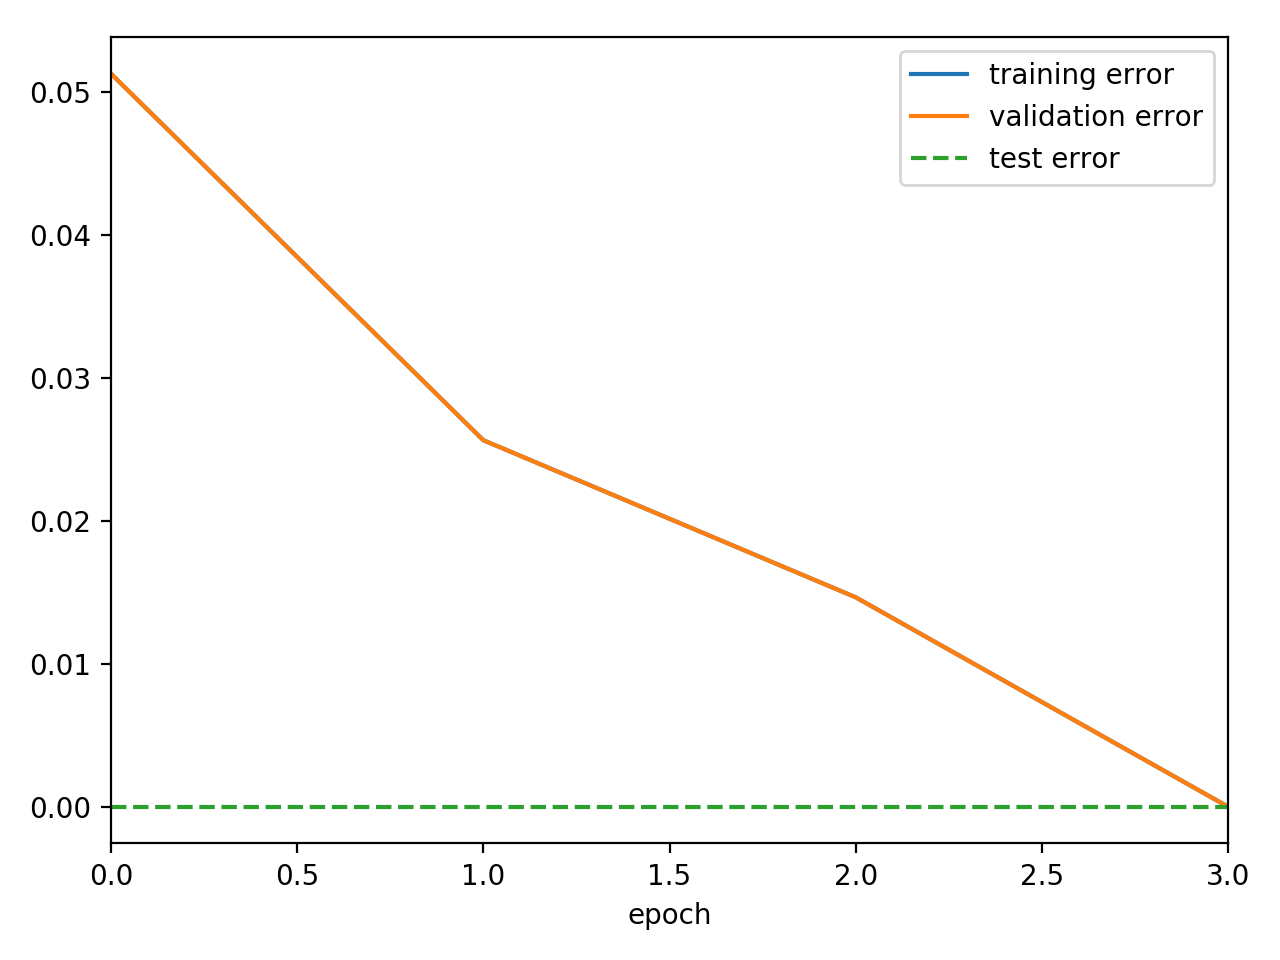
\includegraphics[width=15cm, height=12cm]{AD_LR0015}
\end{figure}

\begin{figure}[h]
\caption{ADAM with learning rate 0.0025}
\centering
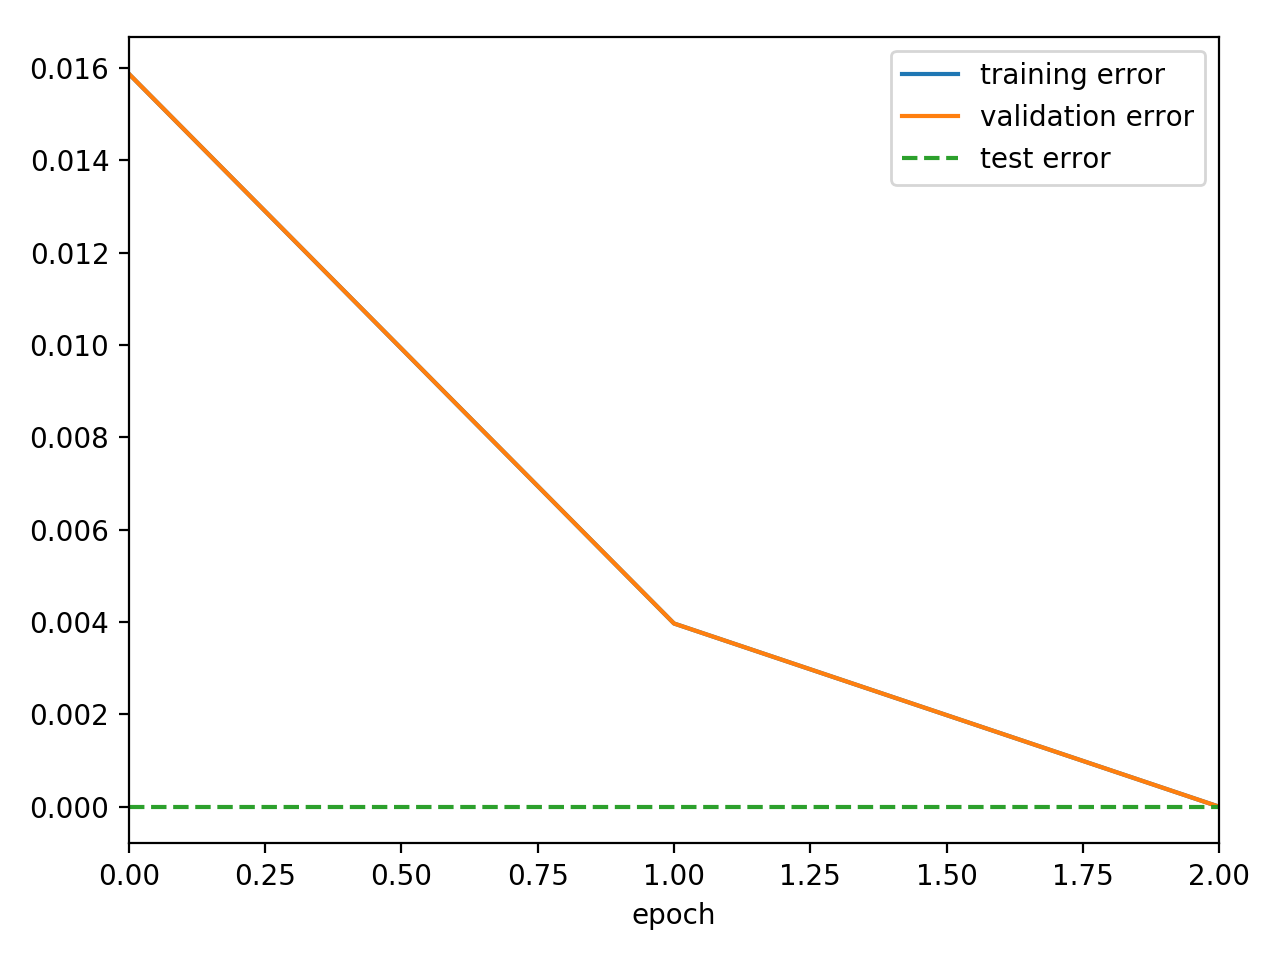
\includegraphics[width=15cm, height=12cm]{AD_LR0025}
\end{figure}

\end{document}